\chapter{O algoritmo de Viola e Jones}\label{cap:viola_jones}

%\chapterprecis{Descrição do algoritmo e detalhamento de seus estágios.}

O algoritmo apresentado por Paul Viola e Michael J. Jones em 2001 \cite{Viola01rapidobject, viola2004robust} e revisado em 2003 \cite{jones2003fast} obteve grande sucesso pela sua relativa simplicidade, rápida execução e notável performance \cite{jensen2008implementing}.

Ele encontra-se implementado na biblioteca OpenCV \cite{bradski2000intel, opencvdocs} e no OpenBR \cite{klontz2013open}. Além de detectar faces, o algoritmo também pode ser treinado para detecção de outras partes do corpo \cite{mustafa2014obscenity} e objetos diversos.

O processo de treino é lento, porém a detecção é bastante rápida. De acordo com \citeonline{omaia2009sistema}, ``este foi o primeiro método de detecção de face em tempo real em vídeo, conseguindo processar até 15 quadros por segundo".

De acordo com \citeonline{zhang2010survey} e \citeonline{Viola01rapidobject}, o algoritmo, na forma como proposto no artigo original, possui baixas taxas de detecção para faces de perfil ou inclinadas. Essa limitação foi tratada pelos autores na revisão de 2003 \cite{jones2003fast} e também por outros pesquisadores, porém essas variantes fogem do escopo deste trabalho.

O detector de faces de Viola-Jones possui quatro estágios: seleção de características Haar-like retangulares, criação da imagem integral, que permite o cálculo rápido das características, treino de classificadores por um algoritmo de aprendizado de máquina baseado no AdaBoost e, por fim, o uso de classificadores em cascata, que descarta as regiões de fundo para focar em áreas mais prováveis de conter uma face.


\section{Características Haar-like retangulares}\label{sec:haar_features}

As características de Haar utilizadas por Viola-Jones, ilustradas na \autoref{fig:haar_like_features}, foram inspiradas nos trabalhos de \citeonline{papageorgiou1998general}, que descreveram características construídas a partir de um conjunto de ondaletas de Haar (Haar wavelets).

\begin{figure}[htbp]
    \centering
    \caption{Características Haar-like}
    \label{fig:haar_like_features}
    \begin{subfigure}[t]{0.2\textwidth}
    \centering
    
\includegraphics{imagens/haar_like_features1.png}
    \caption{}\label{fig:haar_like_features:a}
    \end{subfigure}
    \begin{subfigure}[t]{0.2\textwidth}
    \centering
    
\includegraphics{imagens/haar_like_features2.png}
    \caption{}\label{fig:haar_like_features:b}
    \end{subfigure}
    \begin{subfigure}[t]{0.2\textwidth}
    \centering
    
\includegraphics{imagens/haar_like_features3.png}
    \caption{}\label{fig:haar_like_features:c}
    \end{subfigure}
    \begin{subfigure}[t]{0.2\textwidth}
    \centering
    
\includegraphics{imagens/haar_like_features4.png}
    \caption{}\label{fig:haar_like_features:d}
    \end{subfigure}
\end{figure}

As características Haar-like consistem em um ou mais retângulos adjacentes e são utilizadas para analisar locais específicos em uma janela de detecção. Cada característica resulta em um único valor, calculado através da soma das intensidades dos pixels sob os retângulos brancos subtraída da soma dos valores sob os retângulos pretos, como na \autoref{eq:calc_haar_feature}:
%
\begin{equation} \label{eq:calc_haar_feature}
\Delta = \frac{1}{n}  \sum_{preto}^{n} I(x) - \frac{1}{n}  \sum_{branco}^{n} I(x)
\end{equation}
%
Quanto mais próximo de 1, mais semelhante é a imagem real da característica aplicada.

\begin{figure}[htbp]
    \caption[Exemplo de característica aplicada a uma imagem real]{Exemplo de característica Haar-like retangular de $4\times4$ pixels aplicada a uma imagem real. Pela \autoref{eq:calc_haar_feature}, $\Delta = 0,74 - 0,18 = 0,56$.}
    \label{fig:caract_imagem_real}
    \begin{subfigure}[c]{0.45\textwidth}
    \centering
    \begin{tikzpicture}
    \matrix[square matrix, text=cyan] {
        0 & 0 &|[fill=black]| 1 &|[fill=black]| 1 \\
        0 & 0 &|[fill=black]| 1 &|[fill=black]| 1 \\
        0 & 0 &|[fill=black]| 1 &|[fill=black]| 1 \\
        0 & 0 &|[fill=black]| 1 &|[fill=black]| 1 \\
    };
    \end{tikzpicture}
    \caption{Intensidades ideais}
    \end{subfigure}
    \begin{subfigure}[c]{0.45\textwidth}
    \centering
    \begin{tikzpicture}
    \matrix[square matrix, text=cyan] {
        |[fill=black!20]|0.2 &|[fill=black!20]| 0.2 &|[fill=black!80]| 0.8 &|[fill=black!60]| 0.6 \\
        |[fill=black!10]|0.1 &|[fill=black!30]| 0.3 &|[fill=black!60]| 0.6 &|[fill=black!80]| 0.8 \\
        |[fill=black!20]|0.2 &|[fill=black!10]| 0.1 &|[fill=black!80]| 0.8 &|[fill=black!80]| 0.8 \\
        |[fill=black!20]|0.2 &|[fill=black!10]| 0.1 &|[fill=black!60]| 0.6 &|[fill=black!90]| 0.9 \\
    };
    \end{tikzpicture}
    \caption{Valores reais}
    \end{subfigure}
\end{figure}

Utilizar características é mais vantajoso do que trabalhar com cada pixel da imagem separadamente, pois é menos custoso computacionalmente e elas permitem reconhecer padrões determinados. A característica da \autoref{fig:haar_like_features:b} pode ser utilizada para reconhecer a região dos olhos, que costuma ser mais escura do que a região das bochechas, e a característica 3 pode ser usada para reconhecer a região do nariz, como mostrado na \autoref{fig:julio_haar}.

Existem alternativas mais sofisticadas às características Haar-like, como filtros orientáveis (steerable filters) \cite{freeman1991design, greenspan1994overcomplete}, porém, segundo \citeonline{Viola01rapidobject}, a eficiência de características retangulares fornece ampla compensação por sua flexibilidade limitada.\index{alternativas às características Haar-like}

\begin{figure}[htbp]
   \caption{Características propostas por Lienhart e Maydt}
   \label{fig:lienhart_haar_features}
   \begin{center}
     \scalebox{0.25}{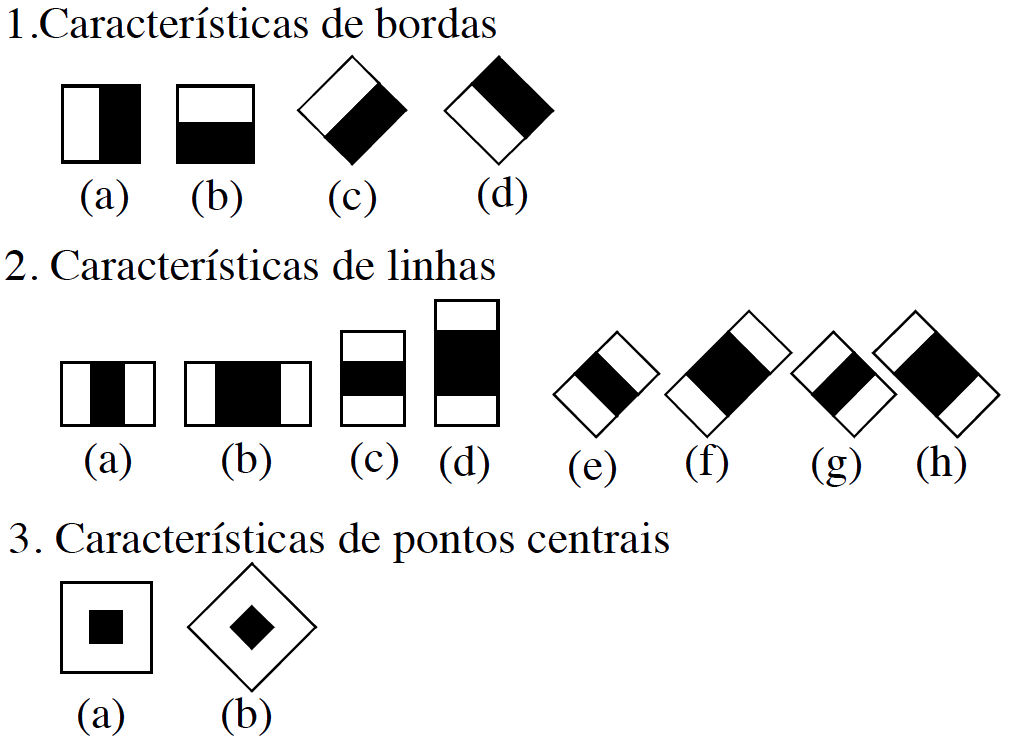
\includegraphics{imagens/lienhart_haar_features.png}}
   \end{center}
\end{figure}

Em \citeonline{lienhart2002extended} foram propostas novas características contendo rotações de \ang{45}, mostradas na \autoref{fig:lienhart_haar_features}. Segundo os autores, o uso dessas características reduziu em 10\%, em média, o número de alarmes falsos. \citeonline{messom2009stream} estenderam essa ideia para rotações de qualquer ângulo, ao custo dos erros de arredondamento.\index{características Haar-like contendo rotação}

\begin{figure}[htbp]
    \caption{Características usadas para detectar olhos e nariz}
    \label{fig:julio_haar}
    \begin{subfigure}[c]{0.3\textwidth}
    \centering
    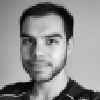
\includegraphics{imagens/julio_haar1.png}
    \caption{}
    \end{subfigure}
    \begin{subfigure}[c]{0.3\textwidth}
    \centering
    
\includegraphics{imagens/julio_haar2.png}
    \caption{}
    \end{subfigure}
    \begin{subfigure}[c]{0.3\textwidth}
    \centering
    
\includegraphics{imagens/julio_haar3.png}
    \caption{}
    \end{subfigure}
\end{figure}

Para uma imagem com resolução de $24\times24$ pixels, pode-se construir dezenas de milhares de características diferentes considerando todas as variações de tamanho e posição das características na \autoref{fig:haar_like_features}. Para calcular todas elas de forma eficiente, é usada uma representação intermediária da imagem, chamada imagem integral.


\section{Imagem Integral}\label{sec:imagem_integral}

O algoritmo da imagem integral, proposto por \citeonline{crow1984summed} para mapeamento de texturas (mipmaps), é capaz de calcular rapidamente a soma dos valores em um subconjunto retangular de uma matriz.

A imagem integral é uma tabela bidimensional do tamanho da imagem original, onde cada elemento equivale à soma de todos os níveis de cinza (intensidades) dos pixels à esquerda e acima do pixel atual, inclusive. Ela pode ser descrita pela \autoref{eq:imagemintegral}:
%
\begin{equation} \label{eq:imagemintegral}
    ii(x,y) = \sum_{{x}'\leq x, {y}'\leq y} i({x}', {y}')
\end{equation}
%
onde $ii(x,y)$ é a imagem integral e $i(x,y)$ é a imagem original.

\begin{figure}[htbp]
    \caption{Imagem ilustrada como matriz de pixels}
    \label{fig:imagem_integral}
    \begin{subfigure}[c]{0.3\textwidth}
    \centering
    \begin{tikzpicture}
    \matrix[square matrix=1.7em] (m){
        0.1 & 0.1 & 0.2 & 0.1 & 0.7 \\
        0.2 & 0.3 & 0.2 & 0.7 & 0.8 \\
        0.1 & 0.4 & 0.3 & 0.3 & 0.1 \\
        0.1 & 0.5 & 0.1 & 0.1 & 0.2 \\
        0.1 & 0.4 & 0.8 & 0.5 & 0.6 \\
    };
    \end{tikzpicture}%
    \caption{Imagem original}
    \end{subfigure}%
    \begin{subfigure}[c]{0.3\textwidth}
    \centering
    \begin{tikzpicture}
    \matrix[square matrix=1.7em, opacity=0.8] (m){
        0.1 & 0.1 & 0.2 & 0.1 & 0.7 \\
        0.2 & 0.3 & 0.2 & 0.7 & 0.8 \\
        0.1 & 0.4 & 0.3 & 0.3 & 0.1 \\
        0.1 & 0.5 & 0.1 & 0.1 & 0.2 \\
        0.1 & 0.4 & 0.8 & 0.5 & 0.6 \\
    };
    \filldraw[fill=yellow, fill opacity=0.2, text opacity=1] (m-2-3.north west) rectangle (m-4-4.south east);% node[pos=.5] {D};
    \fill[blue] (m-1-2.south east) circle(2pt) node[left, font=\small] {\textbf{A}};
    \fill[blue] (m-1-4.south east) circle(2pt) node[right, font=\small] {\textbf{B}};
    \fill[blue] (m-4-2.south east) circle(2pt) node[left, font=\small] {\textbf{C}};
    \fill[blue] (m-4-4.south east) circle(2pt) node[right, font=\small] {\textbf{D}};
    \end{tikzpicture}%
    \caption{Região de interesse}
    \end{subfigure}%
    \begin{subfigure}[c]{0.3\textwidth}
    \centering
    \begin{tikzpicture}
    \matrix[square matrix=1.7em] (m){
        0.1 & 0.2 & 0.4 & 0.5 & 1.2 \\
        0.3 & 0.7 & 1.1 & 1.9 & 3.4 \\
        0.4 & 1.2 & 1.9 & 3.0 & 4.6 \\
        0.5 & 1.7 & 2.5 & 3.7 & 5.3 \\
        0.6 & 2.3 & 3.9 & 5.6 & 8.0 \\
    };
    \filldraw[fill=yellow, fill opacity=0.2] (m-1-2.north west) rectangle (m-1-2.south east);
    \filldraw[fill=yellow, fill opacity=0.2] (m-1-4.north west) rectangle (m-1-4.south east);
    \filldraw[fill=yellow, fill opacity=0.2] (m-4-2.north west) rectangle (m-4-2.south east);
    \filldraw[fill=yellow, fill opacity=0.2] (m-4-4.north west) rectangle (m-4-4.south east);
    \draw[blue,<-,shorten <=1pt] (m-1-2)
    |- +(0.2,0.8)
    node[right] {$ii(A)$};
     \draw[blue,<-,shorten <=1pt] (m-1-4)
    |- +(0.2,0.8)
    node[right] {$ii(B)$};
    \draw[blue,<-,shorten <=1pt] (m-4-2)
    |- +(0.2,-1.4)
    node[right] {$ii(C)$};
    \draw[blue,<-,shorten <=1pt] (m-4-4)
    |- +(0.2,-1.4)
    node[right] {$ii(D)$};
    \end{tikzpicture}%
    \caption{Imagem integral}
    \end{subfigure}%
\end{figure}

Utilizando a imagem integral, a soma dos níveis de cinza de qualquer área retangular pode ser calculada em quatro referências à memória. A soma dos valores na região ABCD da \autoref{fig:imagem_integral} pode ser rapidamente calculada como mostrado na \autoref{eq:ii_calculo_regiao_abcd}:
%
\begin{align} \label{eq:ii_calculo_regiao_abcd}
    \sum_{(x,y) \in ABCD} i(x,y) &= ii(D) + ii(A) - (ii(B) + ii(C))\\
                                 &= 3,7 + 0,2 - (0,5 + 1,7) = 1,7\nonumber
\end{align}

O cálculo de características compostas por dois retângulos (1 e 2 da \autoref{fig:haar_like_features}), requerem seis referências à memória, as características compostas por três retângulos (3) requerem oito acessos e as compostas por quatro retângulos (4) requer nove acessos.


\section{AdaBoost}\label{sec:adaboost}

Apesar do cálculo de cada característica ser rápido, calcular todo o conjunto de características é inviável. Experimentalmente descobriu-se que um classificador eficiente pode ser formado combinando um pequeno subconjunto com apenas as características mais representativas. O algoritmo de Viola-Jones utiliza uma variante do AdaBoost para selecionar essas características e treinar o classificador.

O AdaBoost é um método de aprendizado de máquina, inventado por Yoav Freund e Robert Schapire\cite{freund1997decision}, que combina de forma ponderada vários classificadores fracos com taxa de acerto acima de 50\% para obter um classificador forte.

Um classificador fraco $h_{j}(x,f_{j},p_{j},\theta_{j})$ consiste em uma característica $f_{j}$, um limite $\theta_{j}$, que decide se x deve ser classificado como positivo (uma face) ou negativo (não face), e uma paridade $p_{j}$, que indica a direção da desigualdade:
%
\begin{equation} \label{eq:weak_classifier}
    h_{j}(x,f_{j},p_{j},\theta_{j}) = 
    \begin{cases}
        1 & \text{se } p_{j}f_{j}(x) < p_{j}\theta_{j}\\
        0 & \text{caso contrário}
    \end{cases}
\end{equation}
%
onde $x$ é uma janela de $24\times24$ pixels de uma imagem.

O algoritmo AdaBoost pode ser descrito pelo \autoref{alg:adaboost}. O \refanexo{cap:anexo_adaboost_python} contém uma implementação em Python.

\begin{algorithm}[htbp]
\caption{AdaBoost}
\label{alg:adaboost}
\SetAlgoLined
\LinesNumbered
\Entrada{l imagens com faces $(x_{i}, y_{i}=1), 1 \leq i \leq l$;\newline
m imagens sem faces $(x_{i}, y_{i}=0), l < i \leq n$;\newline
T classificadores fracos}
\Saida{Um classificador forte $H(x)$}
\BlankLine
\tcp{Inicia com uma distribuição uniforme de pesos}
\eSe{$x_{i}$ tem face}{$w_{1,i} \leftarrow \frac{1}{2l}$}{$w_{1,i} \leftarrow \frac{1}{2m}$}
\BlankLine
\tcp{Cada iteração seleciona um único classificador fraco}
\Para{$t \leftarrow 1$ \Ate T}{
    \tcp{Normaliza os pesos}
    $w_{t,i} \leftarrow \frac{w_{t,i}}{\sum_{j=1}^{n} w_{t,i}}$
    \BlankLine
    \tcp{Seleciona o melhor classificador fraco}
    $h_{t}(x) \leftarrow \text{classificador fraco com menor erro } \epsilon_t = \sum_{i}w_i |h_t(x_i,f_t,p_t,\theta_t) - y_i|$
    \BlankLine
    \tcp{Atualiza os pesos \footnotemark}
    \eSe{$x_{i}$ foi corretamente classificado}{$w_{t+1,i} \leftarrow w_{t,i}$}{$w_{t+1,i} \leftarrow w_{t,i}\frac{\epsilon_t}{1-\epsilon_t}$}
}
\BlankLine
\Retorna{
    \begin{equation} \label{eq:strong_classifier}
    H(x) = 
    \begin{cases}
        1 & \text{se } \sum_{t=1}^{T} ln(\frac{1-\epsilon_t}{\epsilon_t}) h_t(x) \geq \frac{1}{2}\sum_{t=1}^{T} ln(\frac{1-\epsilon_t}{\epsilon_t})\\
        0 & \text{caso contrário}
    \end{cases}
    \end{equation}
}
\end{algorithm}
\footnotetext{A lógica está invertida no artigo original. Esse erro foi replicado em diversos outros artigos. Esta versão está correta, pois faz o peso das imagens classificadas erroneamente aumentar.}

Em \citeonline{viola2004robust}, foi construído um classificador a partir de 200 características. Para uma taxa de detecção de 95\%, ele obteve uma taxa de falso-positivos de 1 em 14084 ($1,4\times10^{-4}$ FPR) em um conjunto de dados de teste, como mostra a \autoref{fig:roc_200_features}.

\begin{figure}[htbp]
   \caption{Curva COR para classificador de 200 características}
   \label{fig:roc_200_features}
   \begin{center}
     \scalebox{0.35}{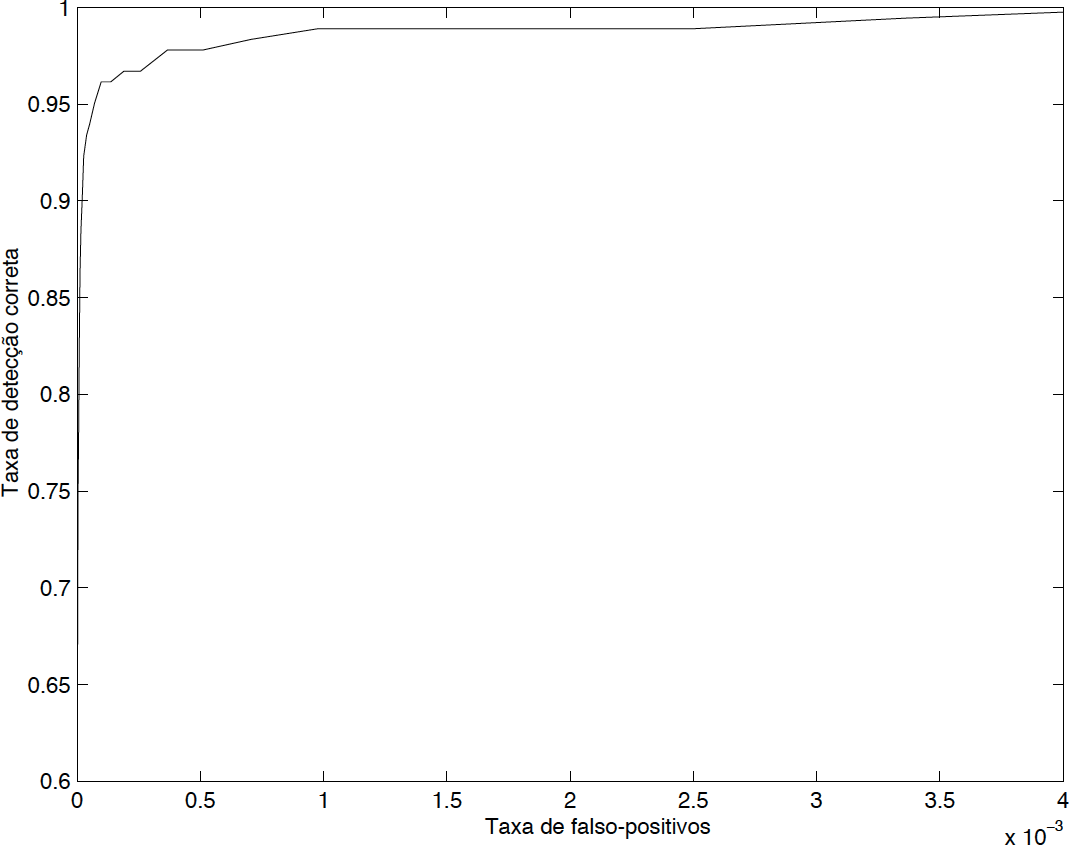
\includegraphics{imagens/roc_200_features.png}}
   \end{center}
\end{figure}
%
Apesar de interessante, esse resultado não é suficiente para muitas aplicações reais tanto pelo tempo gasto quanto pela taxa de falso-positivos.

O classificador processou todas as subjanelas de uma imagem com resolução $384\times288$ pixels em 0,7 segundos em um Intel Pentium III de 700 MHz. Esse valor equivale a 1,43 fps, o que não pode ser considerado tempo real.

Câmeras digitais tiram fotos com vários megapixels de resolução. 
Uma imagem de 1 MP possui $10^6$ pixels, portanto a taxa de falso-positivos desejada nesse caso é de menos de $10^{-6}$.

\section{Classificadores em Cascata}\label{sec:cascade}

\begin{figure}[htbp]
    \caption{Classificadores em cascata}
    \label{fig:cascade_classifiers}
\begin{adjustbox}{max width=\textwidth}
\begin{tikzpicture}[
    font=\scriptsize,
    node distance= 4cm and 3cm,
    arrow/.style = {thick,
                    -stealth},
    decision/.style = {minimum width=#1,
                       diamond, aspect=1.5,
                       text centered,
                       align=center,
                       draw=black},
    process/.style = {minimum width=#1,
                      rectangle,
                      text centered,
                      draw=black},
    startstop/.style = {minimum width=#1,
                        rectangle,
                        rounded corners,
                        text centered,
                        draw=black},
    ]
    
    \node (subjanela) [startstop=5mm] {Subjanela};
    \node (estagio1)  [decision=5mm, right of=subjanela] {Estágio 1\\Face?};
    \node (estagio2)  [decision=5mm, right of=estagio1]  {Estágio 2\\Face?};
    \node (estagio3)  [decision=5mm, right of=estagio2]  {Estágio 3\\Face?};
    \node (detecta)   [process=5mm, right of=estagio3]   {Face detectada};
    
    \DistanciaCentros(estagio1,estagio3){distance}
    \node (rejeita)   [process=\distance, below of=estagio2, node distance=2.0cm]   {Subjanela rejeitada};
    
    \draw [arrow] (subjanela) -- (estagio1);
    \draw [arrow] (estagio1.east) -- node[anchor=south] {Talvez} (estagio2.west);
    \draw [arrow] (estagio2.east) -- node[anchor=south] {Talvez} (estagio3.west);
    \draw [arrow] (estagio3.east) -- node[anchor=south] {Talvez} (detecta.west);
    \draw [arrow] (estagio1.south) -- node[anchor=east] {Não!} (rejeita.north west);
    \draw [arrow] (estagio2.south) -- node[anchor=east] {Não!} (rejeita);
    \draw [arrow] (estagio3.south) -- node[anchor=east] {Não!} (rejeita.north east);
\end{tikzpicture}
\end{adjustbox}
\end{figure}

O classificador em cascata, também chamado de \textit{cascata de atenção} por direcionar a atenção às áreas onde há maior suspeita de haver faces, consiste na concatenação de classificadores gradualmente mais complexos em uma estrutura de cascata.

Cada estágio da cascata contém um classificador forte construído pelo AdaBoost. A função de cada um deles é determinar se uma dada subjanela definitivamente não contém uma face ou talvez contenha uma face. Uma janela é imediatamente descartada se falhar em qualquer estágio. Uma representação do funcionamento da cascata pode ser vista na \autoref{fig:cascade_classifiers}.

Mesmo em fotos com várias pessoas, a maioria das subjanelas avaliadas não contém faces. A ideia chave é que colocar um classificador simples com alta taxa de detecção no início da cascata permite rejeitar as janelas negativas cedo e poupar muito processamento.

\citeauthoronline{viola2004robust} conseguiram treinar um classificador forte, composto por apenas dois classificadores fracos, capaz de detectar 100\% das faces com uma taxa de falso positivo de 50\%. Desta forma, muitas subjanelas de segundo plano puderam ser descartadas com apenas 60 instruções do processador.

A \autoref{fig:roc_200_features_x_cascade} apresenta uma comparação entre um classificador de duzentas características e um classificador em cascata com dez estágios de vinte características cada. O classificador em cascata obteve uma acurácia semelhante com um tempo de execução quase dez vezes menor.


\begin{figure}[htbp]
   \caption{Curvas COR comparando classificador de 200 características com classificador em cascata com 10 estágios de 20 características cada}
   \label{fig:roc_200_features_x_cascade}
   \begin{center}
     \scalebox{0.35}{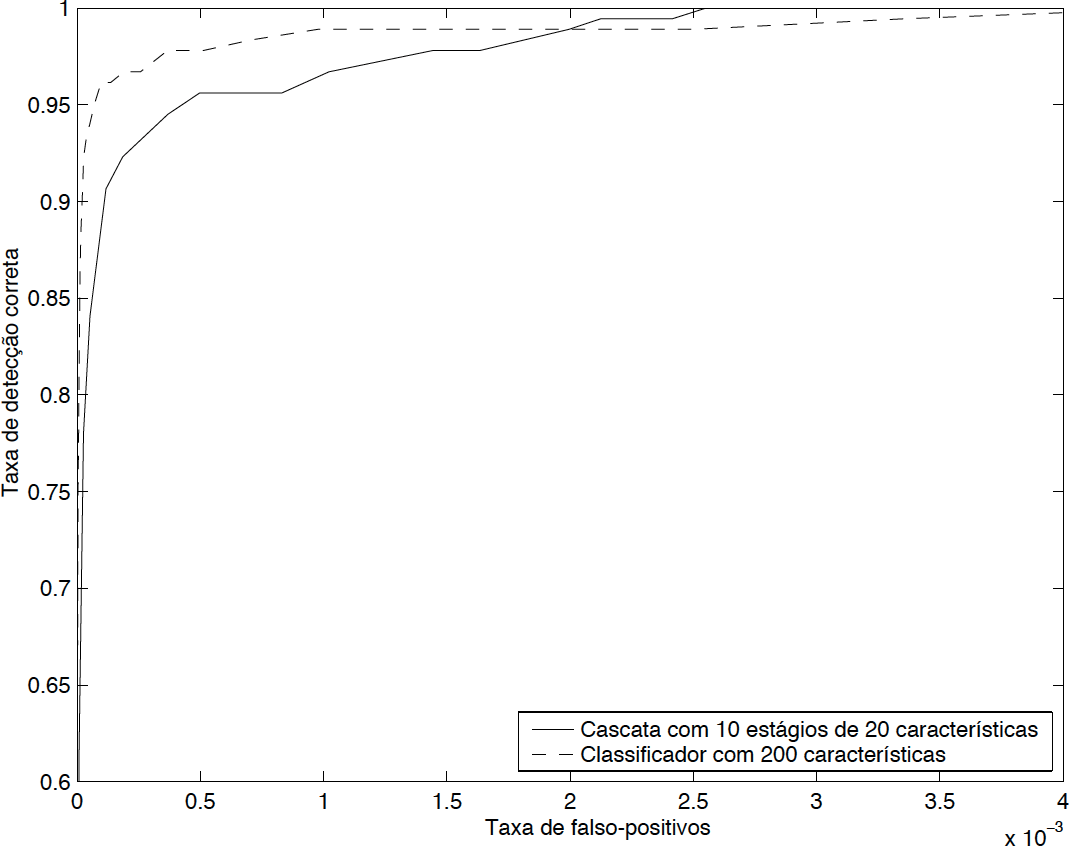
\includegraphics{imagens/roc_200_features_x_cascade.png}}
   \end{center}
\end{figure}


\begin{figure}[htbp]
    \caption{Quatro estágios de um classificador em cascata}
    \label{fig:julio_cascade}
    \begin{subfigure}[t]{0.21\textwidth}
    \centering
    \scalebox{0.21}{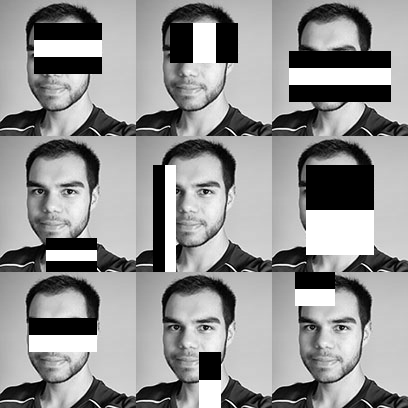
\includegraphics{imagens/cascata_estagio_01.png}}
    \caption{Estágio 1}
    \end{subfigure}
    \begin{subfigure}[t]{0.20\textwidth}
    \centering
    \scalebox{0.21}{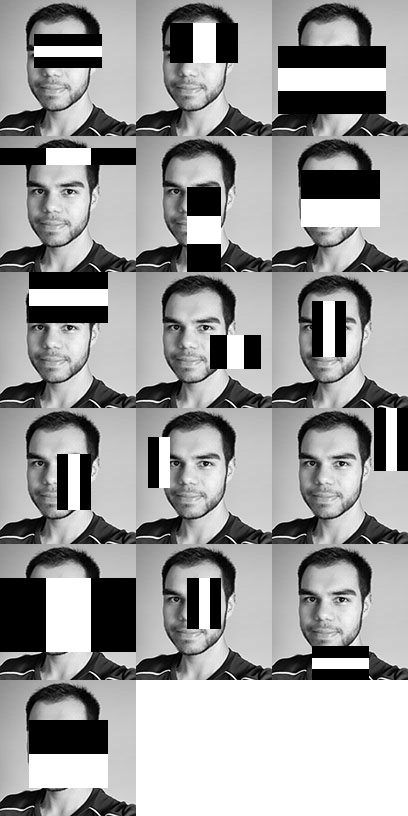
\includegraphics{imagens/cascata_estagio_02.png}}
    \caption{Estágio 2}
    \end{subfigure}
    \begin{subfigure}[t]{0.20\textwidth}
    \centering
    \scalebox{0.21}{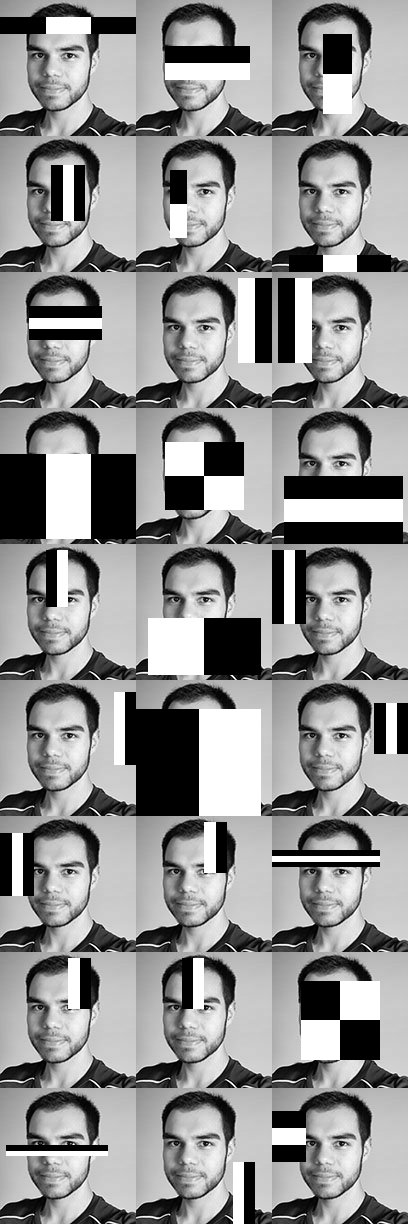
\includegraphics{imagens/cascata_estagio_03.png}}
    \caption{Estágio 3}
    \end{subfigure}
    \begin{subfigure}[t]{0.20\textwidth}
    \centering
    \scalebox{0.21}{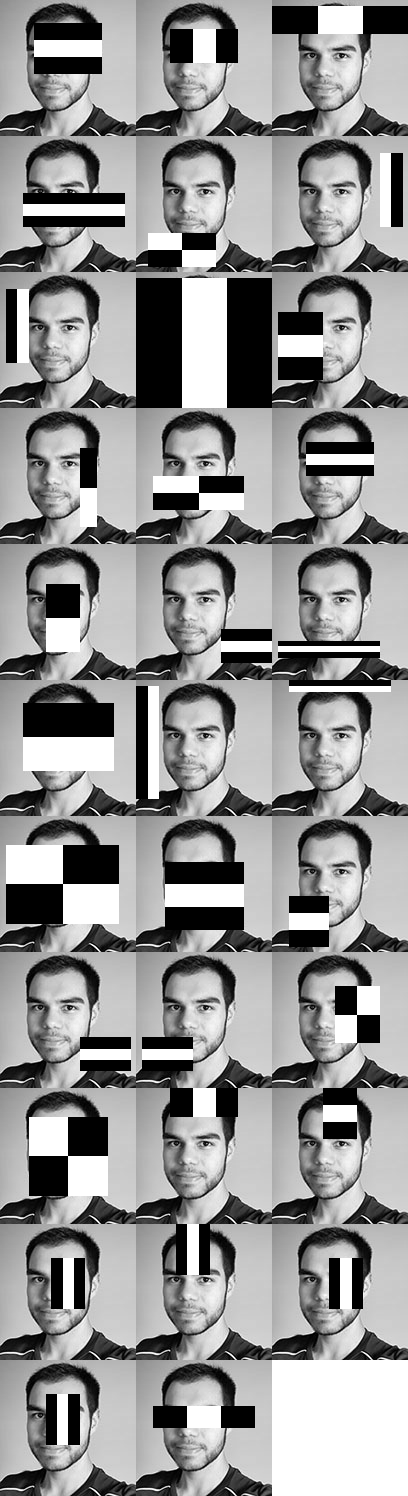
\includegraphics{imagens/cascata_estagio_04.png}}
    \caption{Estágio 4}
    \end{subfigure}
\end{figure}


\subsection{Treino da cascata de classificadores}

A taxa de falso-positivos de uma cascata de classificadores é:
%
\begin{equation} \label{eq:tax_falso_positivos}
F = \prod_{i=1}^{K} f_{i}
\end{equation}
%
onde F é a taxa de falso-positivos da cascata, K é o número de classificadores e $f_{i}$ é a taxa de falso-positivos do i-ésimo classificador.

A taxa de detecção é:
%
\begin{equation} \label{eq:taxa_deteccao}
D = \prod_{i=1}^{K} d_{i}
\end{equation}
%
onde D é a taxa de detecção do classificador, K é o número de classificadores e $d_{i}$ é a taxa de detecção do i-ésimo classificador.

Como explicado na \autoref{sec:adaboost}, a taxa de falso-positivos desejada é da ordem de $10^{-6}$ para uma taxa de detecção acima de 90\%.
O número de estágios da cascata e o tamanho de cada estágio pode ser ajustado para alcançar este objetivo.
Por exemplo, uma cascata de 10 estágios, cada um com 99\% de detecção e um pouco menos de 30\% de falso-positivos, é suficiente.

\begin{algorithm}[htbp]
\caption{Algoritmo de treino do detector em cascata}
\label{alg:train_cascade}
\SetAlgoLined
\LinesNumbered
\Entrada{P: imagens com faces\newline
N: imagens sem faces\newline
$F_{meta}$: taxa desejada de falso-positivos\newline
f: taxa máxima de falso-positivos por estágio\newline
d: taxa mínima de detecção por estágio}
\Saida{Detector de faces treinado}
\BlankLine
$F_{0} \leftarrow 1.0$\\
$D_{0} \leftarrow 1.0$\\
$i \leftarrow 0$
\Enqto{$F_{i} > F_{meta}$}{
    $i \leftarrow i + 1$\\
    $n_{i} \leftarrow 0$ \tcp{quantidade de características do i-ésimo estágio}
    $F_{i} \leftarrow F_{i-1}$
    \BlankLine
    \Enqto{$F_{i} > f \times F_{i1}$}{
        $n_{i} \leftarrow n_{i-1}$\\
        * Usa P e N para treinar um classificador com $n_{i}$ características usando AdaBoost.\\
        * Avalia o classificador atual no conjunto de validação para determinar $F_{i}$ e $D_{i}$.\\
        * Diminui o limite para o i-ésimo classificador até o classificador em cascata atual obter uma taxa de detecção de pelo menos $d \times D_{i-1}$
    }
    \BlankLine
    $N \leftarrow \emptyset$
    \BlankLine
    \Se{$F_{i} > F_{meta}$}{
        Avalia o detector atual no conjunto de imagens sem faces e insere todas as detecções falsas ao conjunto N.
    }
}
\end{algorithm}

Classificadores com mais características obtém maiores taxas de detecção e menos falso-positivos, porém requerem maior tempo de cálculo.